\documentclass[a4paper,10pt]{article}

% Encoding.
\usepackage{geometry}
\usepackage[T2A]{fontenc}
\usepackage[utf8]{inputenc}
\usepackage[english,russian]{babel}

% Code insertion.
\usepackage[outputdir=temp]{minted}

% Math functions.
\usepackage{amsmath}

% Image insertion.
\usepackage{svg}

% No line breaks.
\usepackage[none]{hyphenat}

\title{Задание 1: проектирование CLI}
\author{
	Жилкин Феодор\\
	\and
	Смирнов Александр
}
\date{\today}

\begin{document}


\maketitle

\section*{Поведенческая диаграмма}

\begin{figure}[h]
	\centering
	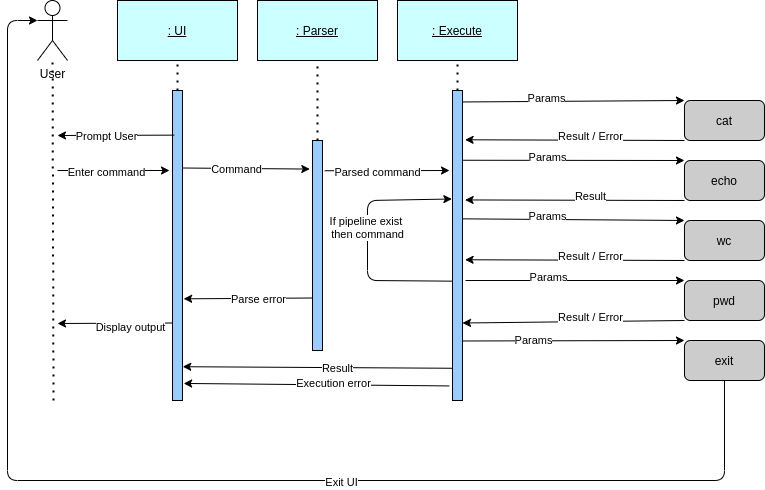
\includegraphics[width=\textwidth]{images/activity_diagram.png}
	\caption{Поведенческая диаграмма}
	\centering
\end{figure}

\newpage

\section*{Диаграмма классов}

\begin{figure}[h]
	\centering
	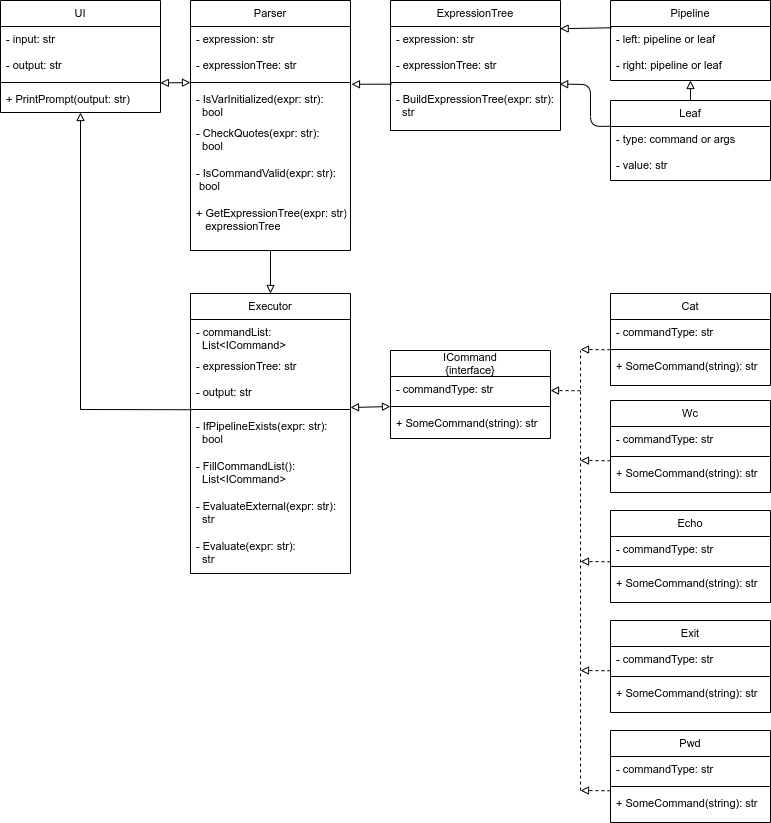
\includegraphics[width=\textwidth]{images/class_diagram.png}
	\caption{Диаграмма классов}
	\centering
\end{figure}

\newpage

\section*{Схема работы}

\begin{itemize}
	\item UI запрашивает у пользователя входные данные
	\item Пользователь вводит команду
	\item Команда попадает в Parser
	      \begin{itemize}
		      \item Parser строит синтаксическое дерево разбора
		            \begin{itemize}
			            \item Представляет сложную команду набором простых команд
			            \item Если встречаем переменную, проверяем, проинициализирована ли она в окружении
			            \item Если встречаем переменную в двойных кавычках, подставляем значение вместо переменной
		            \end{itemize}
		      \item Проверяет команду на валидность
		            \begin{itemize}
			            \item Существует ли команда в \$PATH
			            \item Если команда валидна, передаем её в Execute
			            \item Если команда не валидна, возвращаем ошибку в UI
		            \end{itemize}
	      \end{itemize}
	\item Если в команде присутствует pipeline, то отправляем на исполнение первую команду
	      \begin{itemize}
		      \item Если введённая команда не поддерживается интерпретатором, то исполняем внешнюю команду
		            \begin{itemize}
			            \item Подаём внешней команде аргументы на stdin
			            \item Если команда завершилась с ошибкой, передаём ошибку из stderr в UI
			            \item Если команда завершилась успешно, возвращаем результат работы команды из stdout
		            \end{itemize}
		      \item Если введённая команда поддерживается интерпретатором, то выбираем команду для исполнения
		            \begin{itemize}
			            \item Сравниваем введённую команду с множеством команд интерпретатора
			            \item Если это exit, то выходим из UI
			            \item Подаём команде аргументы на stdin
			            \item Если команда завершилась с ошибкой, передаём ошибку из stderr в UI
			            \item Если команда завершилась успешно, возвращаем результат работы команды из stdout
		            \end{itemize}
		      \item Результат команды передаём в Execute в качестве stdin следующей команде
	      \end{itemize}
	\item Если в команде отсутствует pipeline, то отправляем команду на исполнение и возвращаем результат в UI
\end{itemize}


% \newpage

% \section*{Пример использования}

% Разберём исполнение следующей команды:
% \begin{minted}{bash}
% cat example.txt | wc
% \end{minted}

% \begin{itemize}
%     \item UI запросил у пользователя входные данные ()
% 	\item Пользователь ввёл команду
% 	\item Команда попала в Parser
% 	\item Parser разобрал команду, не нашёл ошибок
% 	\item Parser передал команду в Execute
% 	\item Execute обнаружил pipeline
% 	\item Execute подал первую команду до pipeline на исполнение команде cat с параметром example.txt
% 	\item Команда cat без ошибок выполнилась
% 	\item Execute получил результат "hello world"
% 	\item Execute подал вторую команду wc на исполнение команде wc с параметром "hello world"
% 	\item Команда wc без ошибок выполнилась
% 	\item Execute получил результат 1 2 11
% 	\item Execute передал в UI результат
% 	\item UI отобразил результат
% \end{itemize}


\end{document}
